\documentclass{article}
\usepackage[margin=2.5cm, top=4cm, headheight=25pt]{geometry}
\usepackage{amsmath, amssymb, enumitem, fancyhdr, graphicx}
\usepackage[indent=20pt]{parskip}
\usepackage[hidelinks]{hyperref}
\usepackage{xcolor}
\usepackage{listings}
\usepackage{subcaption}
\usepackage{url}
\usepackage[most]{tcolorbox}
\usepackage{lastpage}
\usepackage{tikz}
\usepackage{circuitikz}

\usetikzlibrary{arrows, positioning}
\tcbuselibrary{listingsutf8} % Support for lstlistings within tcolorbox

\newtcolorbox[auto counter, number within=section]{question}[1][]{%
    colframe=gray!80,                      % Dark gray frame
    colback=gray!5,                       % Light gray background
    coltitle=black,                        % Black title
    title=\textbf{Question~\thetcbcounter}, % Bold title
    fonttitle=\bfseries\large,             % Subtle title font size
    rounded corners,                   % Slightly more rounded corners
    boxrule=0.25mm,                         % Thinner border for a sleek look
    enhanced,                              % Enhanced box features
    attach boxed title to top left={xshift=2mm, yshift=-2mm},
    boxed title style={colframe=gray!80, colback=gray!5, boxrule=0.25mm},
    % Title styling
    #1
}

\bibliographystyle{IEEEtran}
\graphicspath{{./images/}}

% -- Custom Variables --
\def\me{Rajdeep Gill 7934493}
\def\course{ECE 3760}
\def\labsection{A01}

\def\labno{8}
\def\title{Assignment 8: CRC LFSR FSM  Arithmetic in GF(2)}

% -- Styling for code snippets --
\lstset{
    basicstyle=\ttfamily\scriptsize,           % Basic font style
    keywordstyle=\color{blue},            % Keywords color
    commentstyle=\color{gray},            % Comments color
    stringstyle=\color{teal},             % Strings color
    numbers=left,                         % Line numbers on the left
    numberstyle=\tiny\color{gray},        % Line number style
    stepnumber=1,                         % Line number step
    numbersep=10pt,                       % Space between line numbers and code
    backgroundcolor=\color{lightgray!10}, % Background color
    frame=single,                         % Adds a frame around the code
    breaklines=true,                      % Line breaking for long lines
    captionpos=b,                         % Caption position
    showspaces=false,                     % Don't show spaces
    showstringspaces=false                % Don't show spaces in strings
}
\renewcommand{\lstlistingname}{Code Snippet}

\renewcommand{\arraystretch}{1.2} % For less-ugly tables
\setlength\parindent{0pt}

%----- Samples 
% Questions:
%   \begin{question}[title=Custom Question Title]
%       Question details
%   \end{question}

% Tables:
%   \begin{table}[htbp]
%       \centering
%       \caption{Table Caption}
%       \begin{tabular}{ll}
%           \toprule
%           \textbf{Column 1} & \textbf{Column 2} \\
%           \midrule
%           Row 1 & Row 2 \\
%           Row 3 & Row 4 \\
%           \bottomrule
%       \end{tabular}
%   \end{table} 

% Figures:
%   Single figure:
%       \begin{figure}[htbp]
%           \centering
%           \includegraphics[width=0.5\textwidth]{example-image}
%           \caption{Figure Caption}
%       \end{figure}
%   Multiple figures:
%       \begin{figure}[htbp]
%           \centering
%           \begin{subfigure}[b]{0.5\textwidth}
%               \includegraphics[width=\textwidth]{example-image-a}
%               \caption{First subfigure}
%           \end{subfigure}
%           \begin{subfigure}[b]{0.5\textwidth}
%               \includegraphics[width=\textwidth]{example-image-b}
%               \caption{Second subfigure}
%           \end{subfigure}
%           \caption{Main figure}
%       \end{figure}

\begin{document}

% --------------------------------------------------------------------------------
% TITLE
% --------------------------------------------------------------------------------

\begin{center}
    \huge \title

    \vspace{2mm}
    \hrule

    \vspace{4mm}
    \large \me

    \vspace{2mm}
    \large \course~\labsection

    \vspace{2mm}
    \today
\end{center}

\vspace{4mm}

% --------------------------------------------------------------------------------
% END TITLE
% --------------------------------------------------------------------------------

\newpage


\vspace{1cm}
\newpage

\pagestyle{fancy}
\fancyhead[L]{\large Assignment \labno}
\fancyhead[R]{\large \me}

\fancyfoot[C]{Page \thepage~of~\pageref{LastPage}}

% --------------------------------------------------------------------------------
% BODY
% --------------------------------------------------------------------------------

\section{Part 1}
The polynomial representation for a 3-bit maximal length LFSR is $x^3 + x^2 + 1$. Since it is 3-bits, there are 7 non-zero states and 1 zero state. 

We can verify this by doing the state transition and see if all 7 non-zero states are visited before returning to the initial state.

We will have the taps at bit's 0 and 1, so that the new bit that is shifted in is the XOR of bit 0 and bit 1.
\begin{align*}
    s_2 s_1 s_0 \rightarrow s_{new} s_2 s_1, \quad s_{new} = s_1 \oplus s_0 \\
    \text{Start at: } s_2 s_1 s_0 = 100 &\rightarrow 010 \\
    010 &\rightarrow 101 \\
    101 &\rightarrow 110 \\
    110 &\rightarrow 111 \\
    111 &\rightarrow 011 \\
    011 &\rightarrow 001 \\
    001 &\rightarrow 100 \\
    100 &\rightarrow 010 \\
\end{align*}

We see that all 7 non-zero states are visited and will repeat the sequence. The zero-state will continously visit itself. The LSFR would look like the following:
\begin{figure}[ht!]
    \centering
    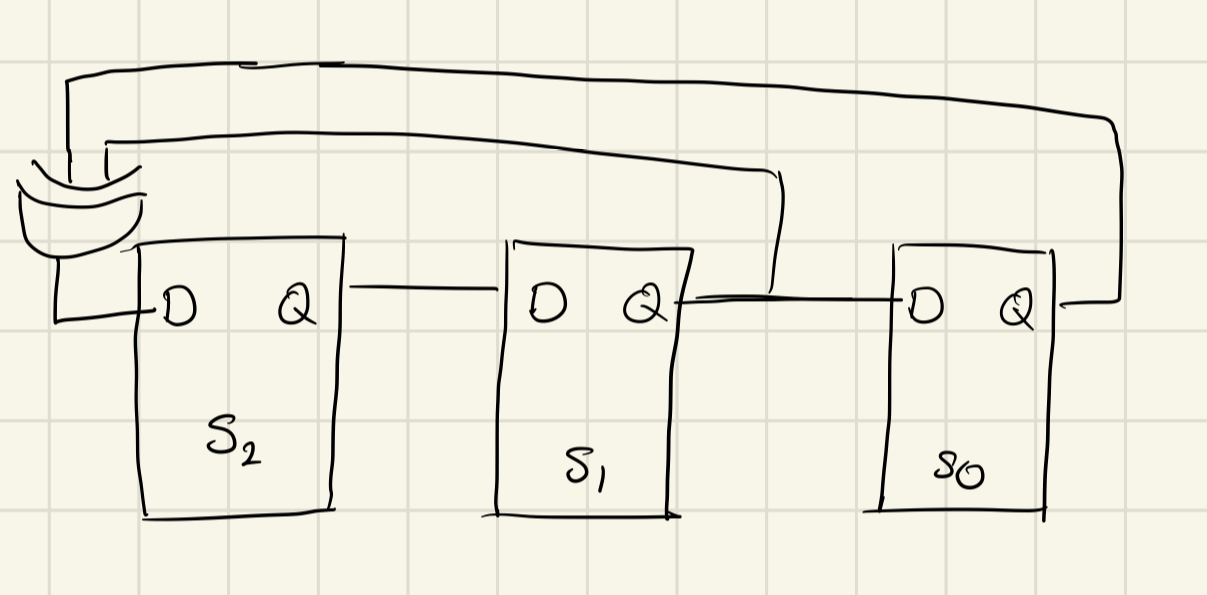
\includegraphics[width=0.6\textwidth]{image.png}
    \caption{LFSR Diagram}
\end{figure}

\textbf{Sender Side Operation:}

We can divide 1011 into 1000 0000, and we get our remainder
\begin{align*}
    1000 0000 = 128, \quad 1011 = 11 \\
    128 \div 11 = 11 \text{ remainder } 7 \\
    \text{Remainder: } 7 = 0111
\end{align*} 

We want to add to our original message to make the remainder 0, so we add (11-7) = 4 to the original message.
\begin{align*}
    1000 0000 + 0100 = 1000 0100
\end{align*}

Now we send this msg over to the receiver and if there is no remainder, then the message should be correct.

\textbf{Receiver Side Operation:}

On the receiver side, we divide the received message 1000 0100 by 1011 and determine if the remainder is 0. If the received message has a supposed error, and a bit-flip occurs, the remainder will not be 0.

Verifying this:
\begin{align*}
    1000 0100 = 132, \quad 1011 = 11 \\
    132 \div 11 = 12 \text{ remainder } 0
\end{align*}

If bitflip occurs, we can see that the remainder will not be 0.
\begin{align*}
    10\mathbf{1}0 0100 = 164, \quad 1011 = 11 \\
    164 \div 11 = 14 \text{ remainder } 10
\end{align*}




\textbf{What does ethernet do on a CRC error? What does WiFi do?
What does ethernet do on NO CRC error? What does WiFi do?
}

On a CRC error on both ethernet and WiFi, the frame is dropped and the receiver sends a NAK to the sender to resend the frame. Depending on the protocol, the sender may resend the frame after a timeout period, or resend on a NAK.

On no CRC error, the frame is accepted and the receiver sends an ACK to the sender to confirm that the frame was received. 

Wi-Fi would have more error checking as compared to ethernet, as the wireless medium is more prone to errors.   
% --------------------------------------------------------------------------------
% END BODY
% --------------------------------------------------------------------------------

\end{document}
